\documentclass{article}
\setcounter{secnumdepth}{0}
\usepackage[utf8]{inputenc}
\usepackage{xcolor}
\usepackage{color}
\usepackage{caption}
\usepackage{enumitem}
\usepackage[colorlinks = true,
            linkcolor = blue,
            urlcolor  = blue,
            citecolor = blue,
            anchorcolor = blue]{hyperref}
\usepackage{hyperref, todonotes}


\title{Environment mapping with a mobile robot \\
\Large MSc thesis diary}
\author{Laszlo Debreczeni}
\date{March 2024 -- December 2024}
\graphicspath{ {./images/} }

\begin{document}
\maketitle

\tableofcontents
\newpage

\section{May 28 -- June 4}
\section{May 21 -- May 28}
\section{May 14 -- May 21}
\section{May 07 -- May 14}
\section{April 30 -- May 07}
\subsection{Reading}
Some links on neural 3D maps:
\begin{itemize}
\item NerfNavigation: Vision-Only Robot Navigation in a Neural Radiance World, \url{https://mikh3x4.github.io/nerf-navigation/}
\item Motion Planning with Implicit Neural Representations of Geometry, \url{https://neural-implicit-workshop.stanford.edu/}
\item Splat-Nav: Safe Real-Time Robot Navigation in Gaussian Splatting Maps, \url{https://arxiv.org/abs/2403.02751}
\item SplaTAM: Splat, Track \& Map 3D Gaussians for Dense RGB-D SLAM\url{https://spla-tam.github.io/}
\item \url{https://github.com/zubair-irshad/Awesome-Implicit-NeRF-Robotics?tab=readme-ov-file#planningnavigation}
\end{itemize}


\section{April 23 -- April 30}

\subsection{Reading}
Literature search about 3D map representations for robot/drone navigation: point cloud map, voxel map, triangle mesh map, 3DGS map, topological map. Which one is the best for 3D camera-based navigation? Which ones can we create with the Turtlebot's sensors?

Some links on traditional 3D maps:
\begin{itemize}
\item Octomap: \url{https://octomap.github.io/}
\item Voxblox: Oleynikova - Voxblox: Incremental 3D Euclidean Signed Distance Fields for On-Board MAV Planning, 
\item VoxboxPlanning: \url{https://github.com/ethz-asl/mav_voxblox_planning}
\item MeshNavigation \url{https://github.com/naturerobots/mesh_navigation}
\item RTAB-Map: \url{https://introlab.github.io/rtabmap/}
\item maplab, maplab 2.0 \url{https://maplab.asl.ethz.ch/docs/master/index.html}
\end{itemize}

\section{April 16 -- April 23}

\subsection{Tasks}
\begin{itemize}
\item person detector + estimate 3D position of person
\item try DepthAI RTAB-Map ROS \url{https://github.com/luxonis/depthai-ros/blob/humble/depthai_ros_driver/launch/rtabmap.launch.py}
\item Optional: try RTAB-MAP iOS \url{https://apps.apple.com/ca/app/rtab-map-3d-lidar-scanner/id1564774365}
\item try to load and continue a SPAI map
\end{itemize}
\newpage


\section{April 9 -- April 16}
\subsection{Reading}
\begin{itemize}
\item 3D Gaussian Splatting, \url{https://repo-sam.inria.fr/fungraph/3d-gaussian-splatting/}
\end{itemize}

\subsection{Tasks}
\begin{itemize}
\item SPAI point cloud map saving and loading, SPAI localization \todo[color=green!30]{DONE}
\item SPAI keyframe+pose saving \todo[color=green!30]{DONE}
\item SPAI mesh saving (optional, if possible) \todo[color=green!30]{DONE}
\item convert SPAI dataset to NerfStudio dataset, reconstruct your room with NerfStudio's gsplat implementation \todo[color=blue!30]{IN PROGRESS}
\item Can you write a script that converts a SPAI dataset into an input dataset for the original 3DGS?\url{https://github.com/graphdeco-inria/gaussian-splatting} Alternatively, can you create a script that converts a NerfStudio dataset to an input dataset for the original 3DGS?
\item try a 3D Gaussian Splatting reconstruction of your room (requires GPU) 
\item try SuperSplat 3DGS editor (for your LumaAI model) \url{https://playcanvas.com/supersplat/editor}
\item try Web-based 3DGS viewer \url{https://github.com/mkkellogg/GaussianSplats3D}
\end{itemize}

\subsection{Achievements}
\begin{itemize}
    \item SPAI point cloud map can be saved by the mapping example. We can export optimized point clouds in ply and pcd formats with \verb|sai-cli|
    \item I could not figure out how could we load and visualize the saved point cloud map yet.
    \item The keyframes and poses can be extracted from the mapping with the help of \verb|sai-cli process|. It saves the keyframes as images and the corresponding 3D points.
    \item The mesh cannot be saved by the pure SDK examples. A video can be used to create the mesh on it and a map can be loaded for the example.
    \item When trying to use the nerfstudio's splatfacto model (Gaussian Splatting), the dromni's docker image throws a CUDA error. The nerfstudio's official image throws this error:\par
    assert block\_width \verb|>| 1 and block\_width \verb|<|= 16, "block\_width must be between 2 and 16"
    AssertionError: block\_width must be between 2 and 16\par
    It is a problem with nerfstudio and/or gsplat. I tried installing older gsplat versions but the problem remained.
\end{itemize}

Gabor: point clouds can be opened and edited by MeshLab or CloudCompare
\newpage


\section{March 28 -- April 9}
\subsection{Reading}
\begin{itemize}
    \item read about neural radiance fields \url{https://www.youtube.com/@thenerfguru}
    \item read about 3D Gaussian Splatting \url{https://www.youtube.com/watch?v=VkIJbpdTujE}
\end{itemize}

\subsection{Tasks}
\begin{itemize}
\item try LumaAI \url{https://lumalabs.ai/} with iPhone RGBD \todo[color=green!30]{DONE}
\item convert SPAI dataset to NerfStudio dataset (SPAI script does that) \todo[color=green!30]{DONE}
\item optionally try a NeRFStudio reconstruction of your room (requires GPU) \todo[color=green!30]{DONE}
\end{itemize}

\subsection{Achievements}
\begin{itemize}
    \item LumaAI: \url{https://lumalabs.ai/capture/00CC75E0-E9C1-42C2-8530-C8D8995CF6A9}
    \item SPAI dataset to NeRFStudio dataset: \verb|sai-cli| command can do that
    \item For the room reconstruction see the previous week's achievements
\end{itemize}

\newpage



\section{March 21 -- March 28}
\subsection{Tasks}
\begin{itemize}
\item Create own ROS2 workspace and create an own ROS2 node \url{https://docs.ros.org/en/foxy/Tutorials/Beginner-Client-Libraries/Creating-A-Workspace/Creating-A-Workspace.html} \todo[color=green!30]{DONE}
\item test SpectacularAI SDK \url{https://github.com/SpectacularAI/sdk-examples} \todo[color=green!30]{DONE}
\item VIO record, replay, visu \url{https://github.com/SpectacularAI/sdk-examples/tree/main/python/oak} \todo[color=green!30]{DONE}
\item ROS wrapper: \url{https://github.com/SpectacularAI/sdk-examples/tree/main/python/oak/ros2} \todo[color=green!30]{DONE}
\item Mapping ROS \url{https://github.com/SpectacularAI/sdk-examples/blob/main/python/oak/mapping_ros.py}: This works only with ROS1!
\item create a point cloud reconstruction of your room
\url{https://www.youtube.com/watch?v=n34dt-Ag1Yo} \todo[color=green!30]{DONE}
\end{itemize}

\subsection{Achievements}
\begin{itemize}
    \item Unfortunately, due to HDD crash and reinstall, the project is delayed by one week. The same tasks are valid for the next week. The solution was to buy a high speed, more reliable external HDD (ADATA HD650 in my case)
    \item A basic ROS2 workspace with packages containing nodes has been created \url{https://github.com/K0pasz/thesis_ros2_test_workspace}
    \item When I try out the SpectecularAI Python examples they log onto the terminal "SpectacularAI WARN: Dropping frames!
SpectacularAI WARN:   VIO may be running too slow, data is being input too fast, or IMU samples are missing / time-offset from frames. (buffer size 10)". SOLUTION: The problem was that the IMU's firmware version was too old. Had to update it, but the documentation is extremely poor about it. What I did: cloned \url{https://github.com/luxonis/depthai-python}, then ran \verb|python3 examples/install_requirements.py| and \verb|python3 examples/IMU/imu_firmware_update.py| which successfully updated the IMU's firmware.
    \item After the successful firmware update, I tried different Spectacular AI examples.
    \item IMU visualization:\par
    \begin{minipage}{\linewidth}
        \centering
        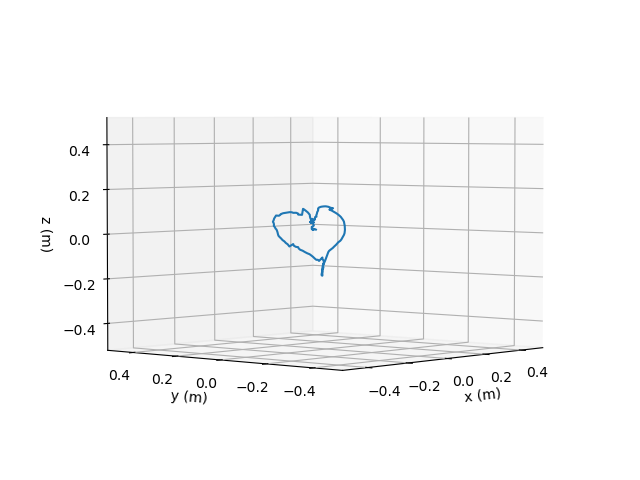
\includegraphics[width=1\linewidth]{spectacular_ai_vio_visu.png}
        \captionof{figure}{IMU visualization}
    \end{minipage}
    \item 3D Pen: if you cover the camera with your hand, you can draw in the air. Video: videos/spectacular\_ai\_3d\_pen.webm
    \item If you want to make the \verb|mapping_visu.py| work, you have to comment out a several lines inside \verb|OpenGL/contexdata.py|:
    \begin{verbatim}
        def getContext( context = None ):
    """Get the context (if passed, just return)
    
    context -- the context ID, if None, the current context
    """
    if context is None:
        context = platform.GetCurrentContext()
        # if context == 0:
        #     from OpenGL import errorS
        #     raise error.Error(
        #         """Attempt to retrieve context when no valid context"""
        #     )
    return context
    \end{verbatim}
    After this, it should work like a charm:\par
    \begin{minipage}{\linewidth}
        \centering
        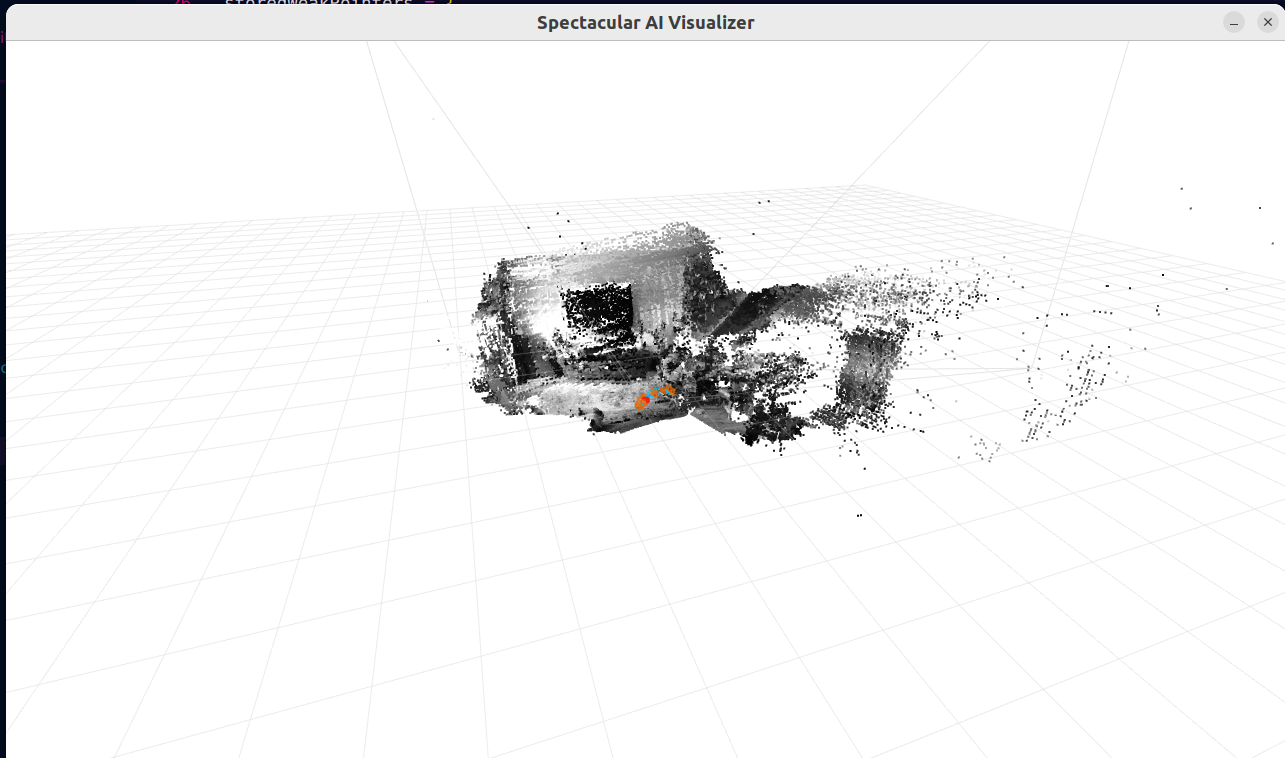
\includegraphics[width=1\linewidth]{spectacular_ai_mapping_visu.png}
        \captionof{figure}{Mapping visualization}
    \end{minipage}
    \item Mapping AR: it can create a mesh and point cloud representation of the surroundings:\par
    \begin{minipage}{\linewidth}
        \centering
        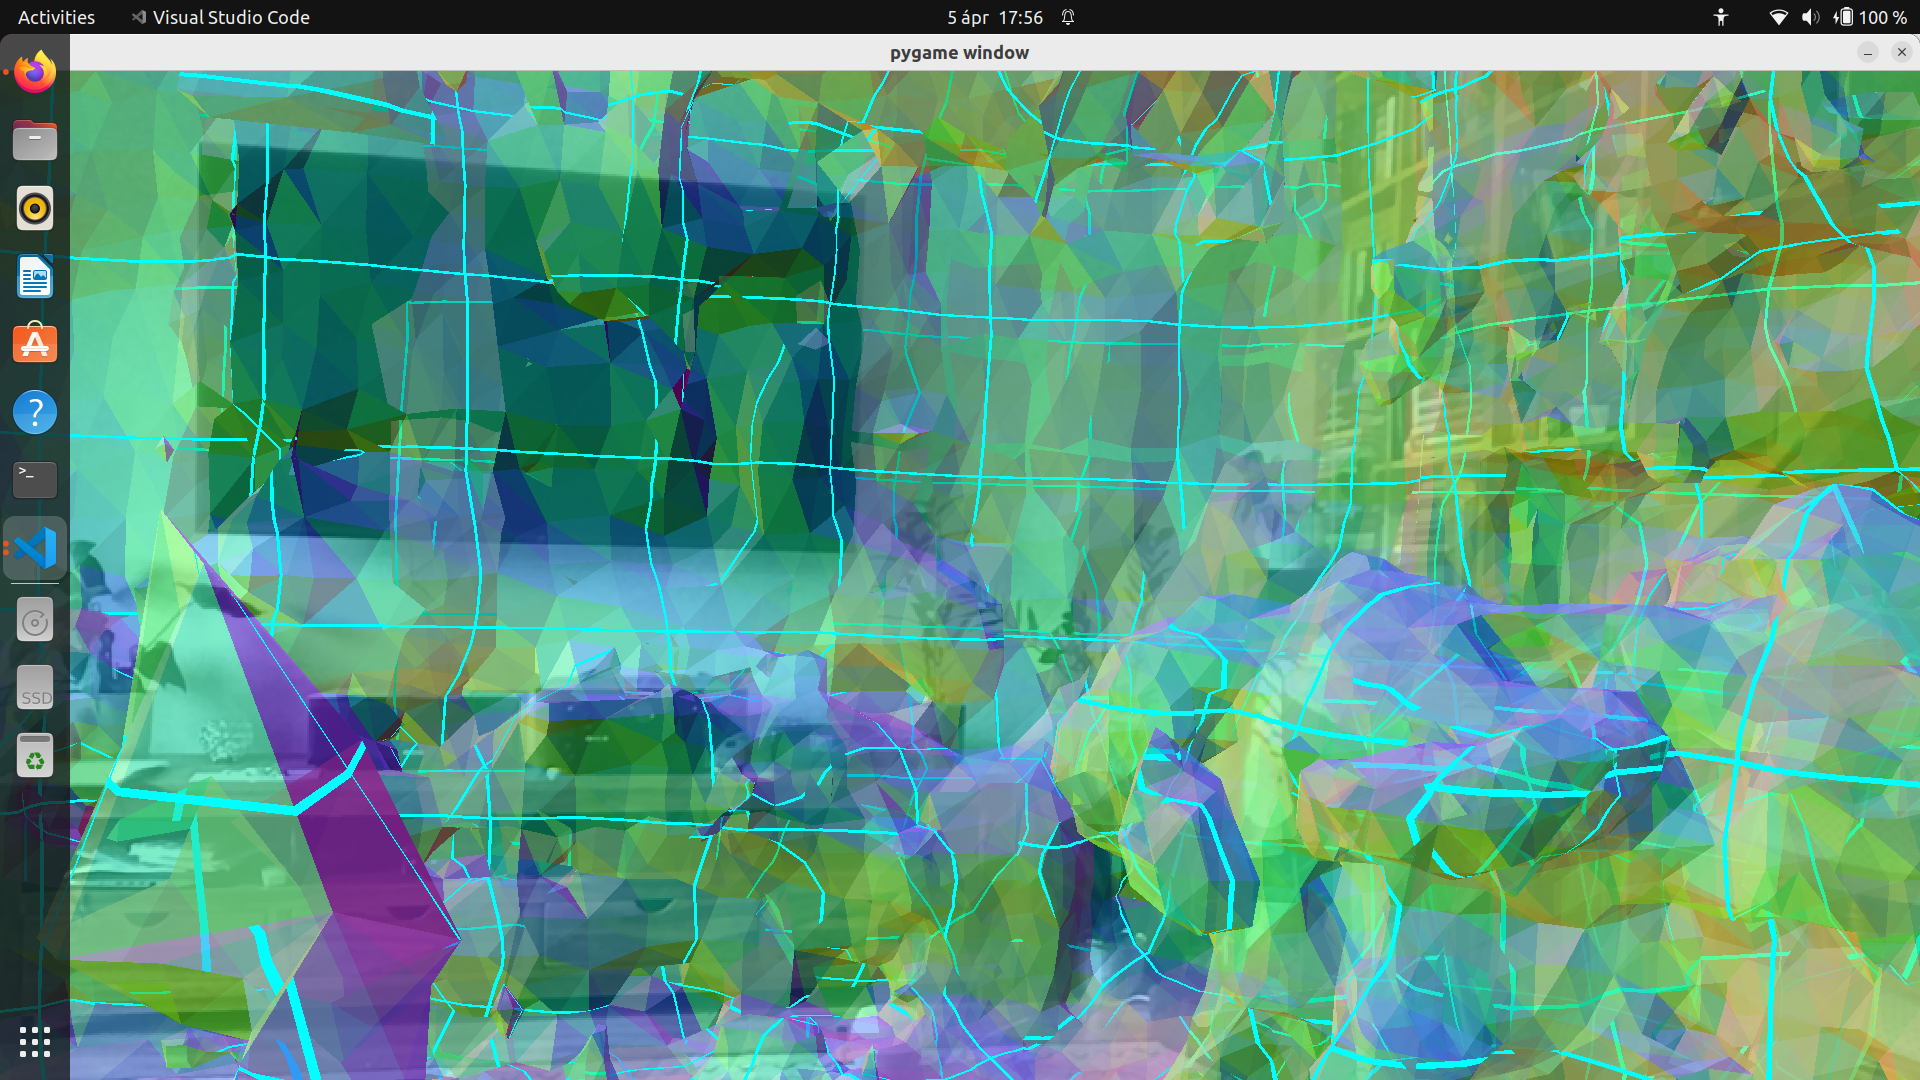
\includegraphics[width=1\linewidth]{spectacular_ai_mapping_ar_mesh1.png}
        \captionof{figure}{Mapping AR with mesh}
    \end{minipage}
    \par
    \begin{minipage}{\linewidth}
        \centering
        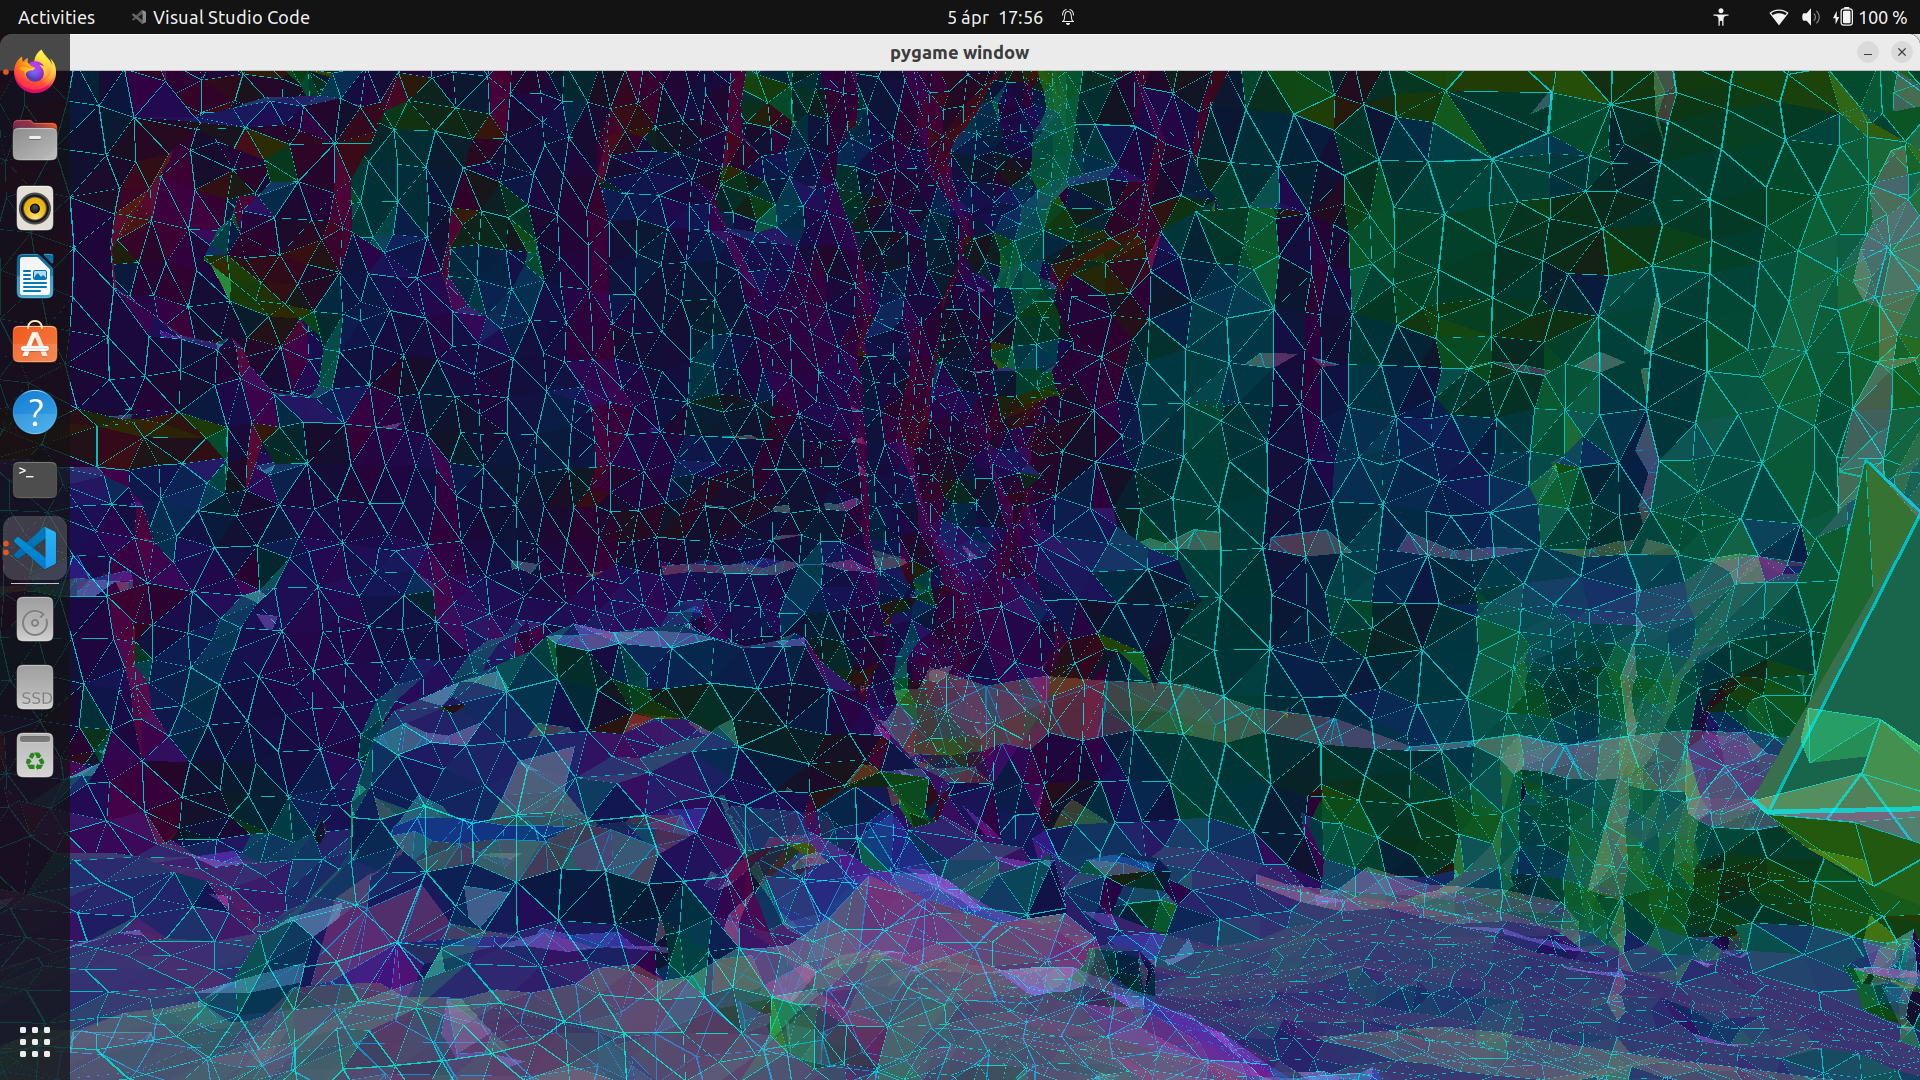
\includegraphics[width=1\linewidth]{spectacular_ai_mapping_ar_mesh2.png}
        \captionof{figure}{Mapping AR with mesh}
    \end{minipage}
    \par
    The point cloud representation was more informative:\par
    \begin{minipage}{\linewidth}
        \centering
        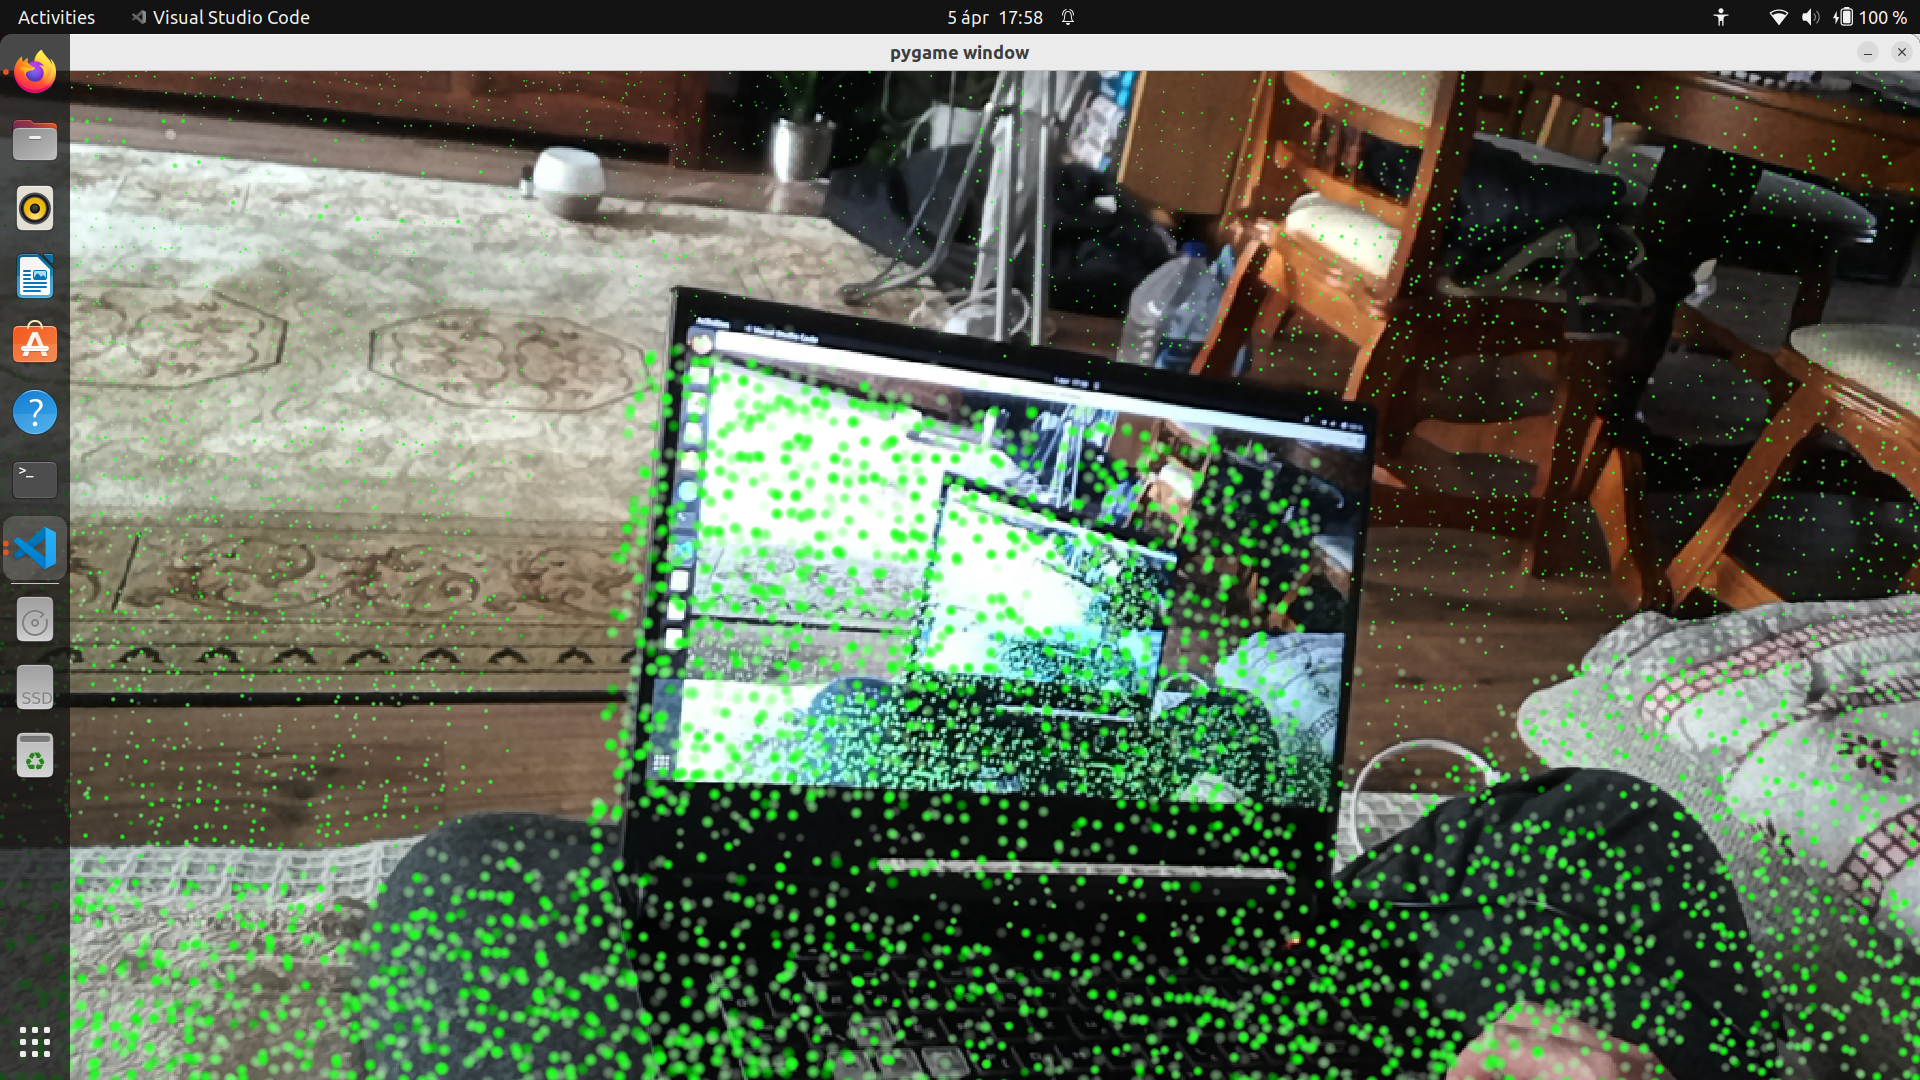
\includegraphics[width=1\linewidth]{spectacular_ai_mapping_ar_pc1.png}
        \captionof{figure}{Mapping AR with point cloud}
    \end{minipage}
    \par
    \begin{minipage}{\linewidth}
        \centering
        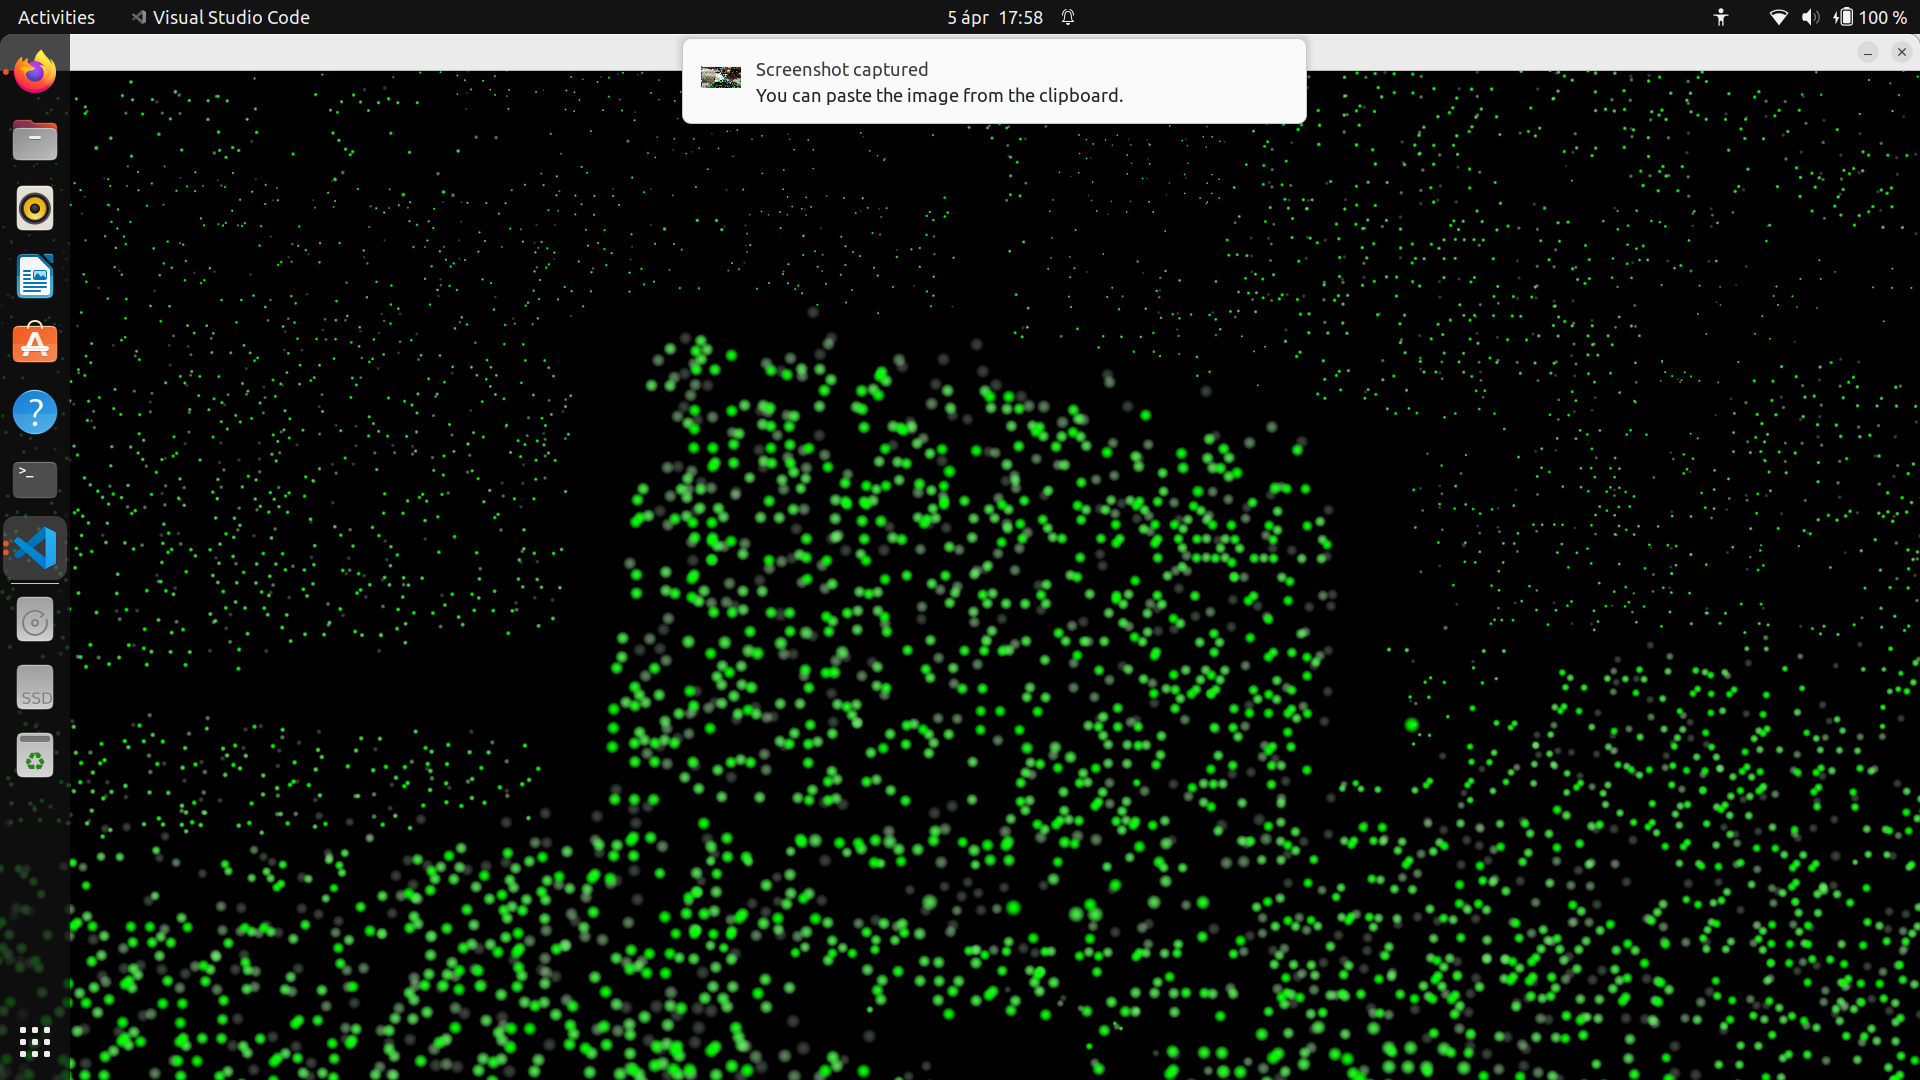
\includegraphics[width=1\linewidth]{spectacular_ai_mapping_ar_pc2.png}
        \captionof{figure}{Mapping AR with point cloud}
    \end{minipage}
    \par
    \item There is an example where ros2 is used for mapping and you can view the created point cloud in RViz:\par
    \begin{minipage}{\linewidth}
        \centering
        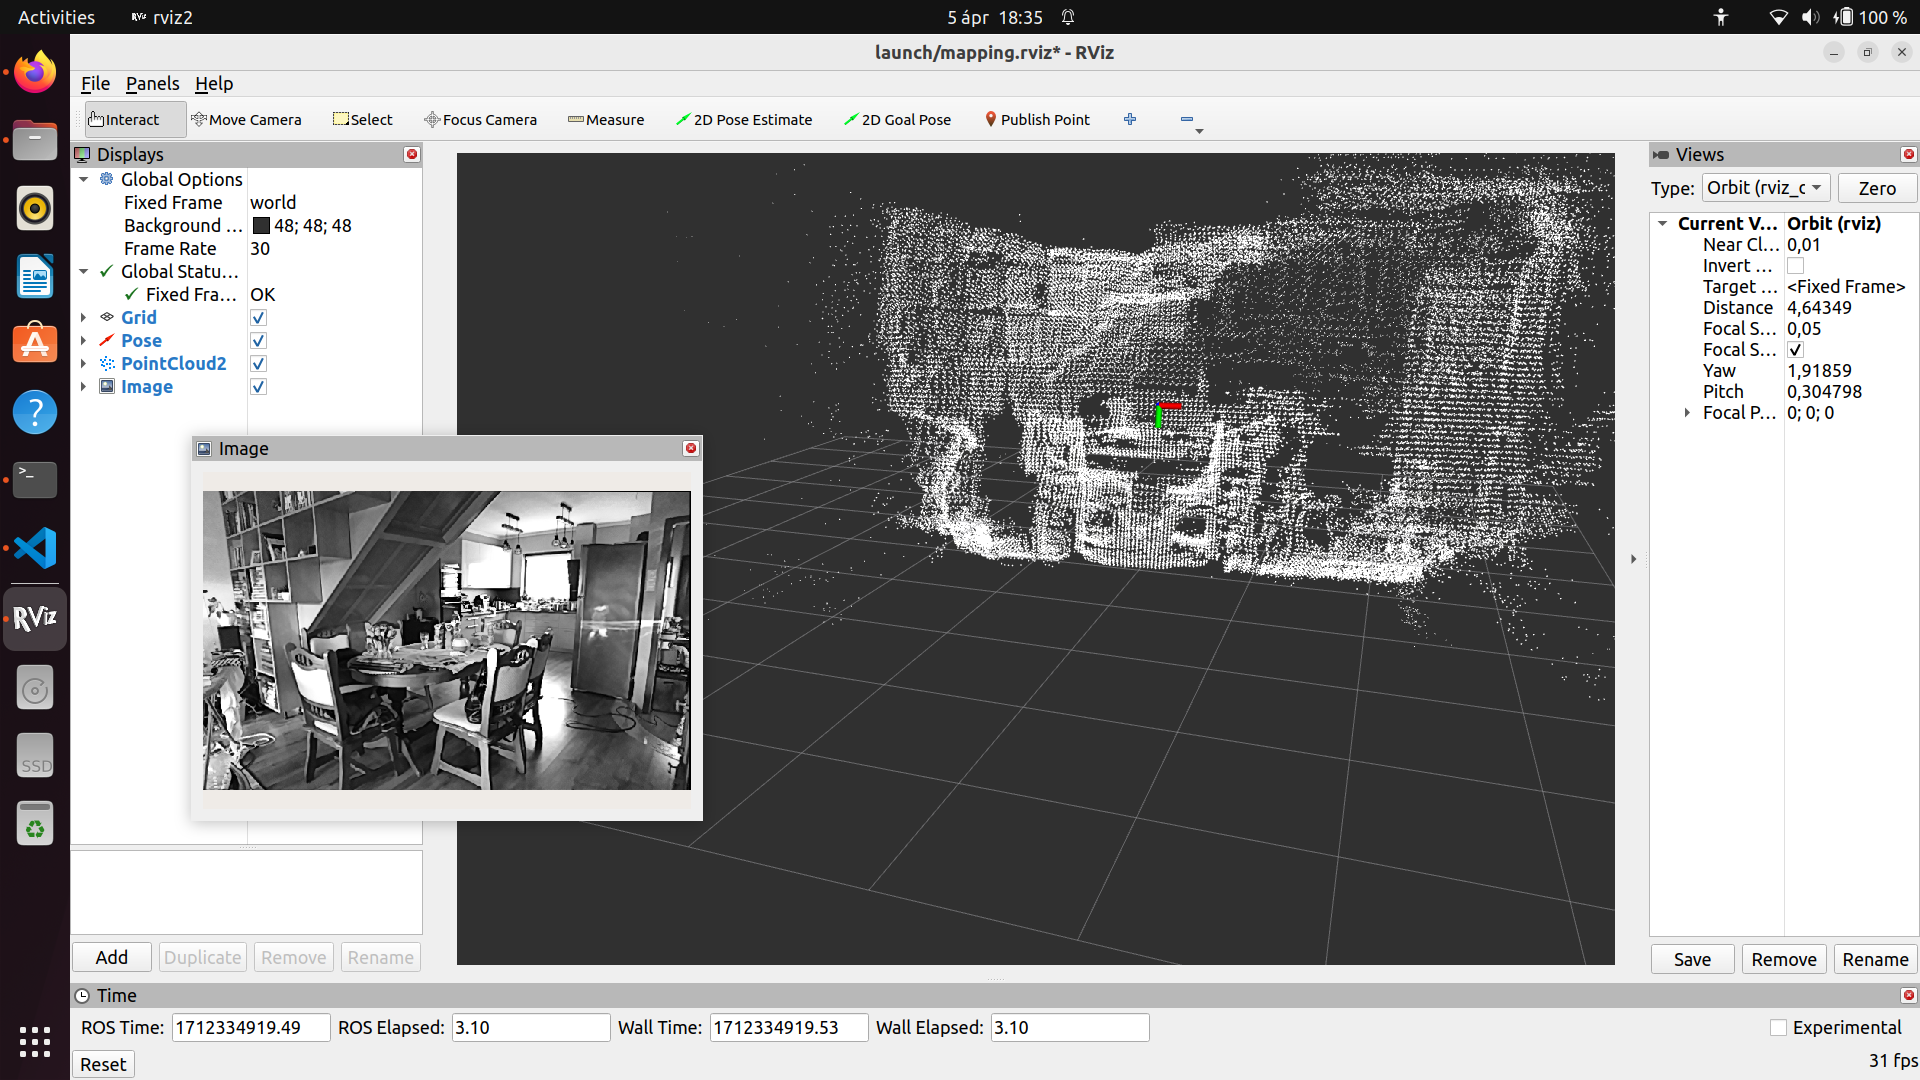
\includegraphics[width=1\linewidth]{spectacular_ai_mapping_ros2.png}
        \captionof{figure}{Mapping with ROS2 and RViz}
    \end{minipage}\par
    You can see the chairs, table and fridge clearly, this works awesome!
    \item One of the most spectacular example is the one that uses depthai. It can detect objects and place them in space with absolute positions:\par
    \begin{minipage}{\linewidth}
        \centering
        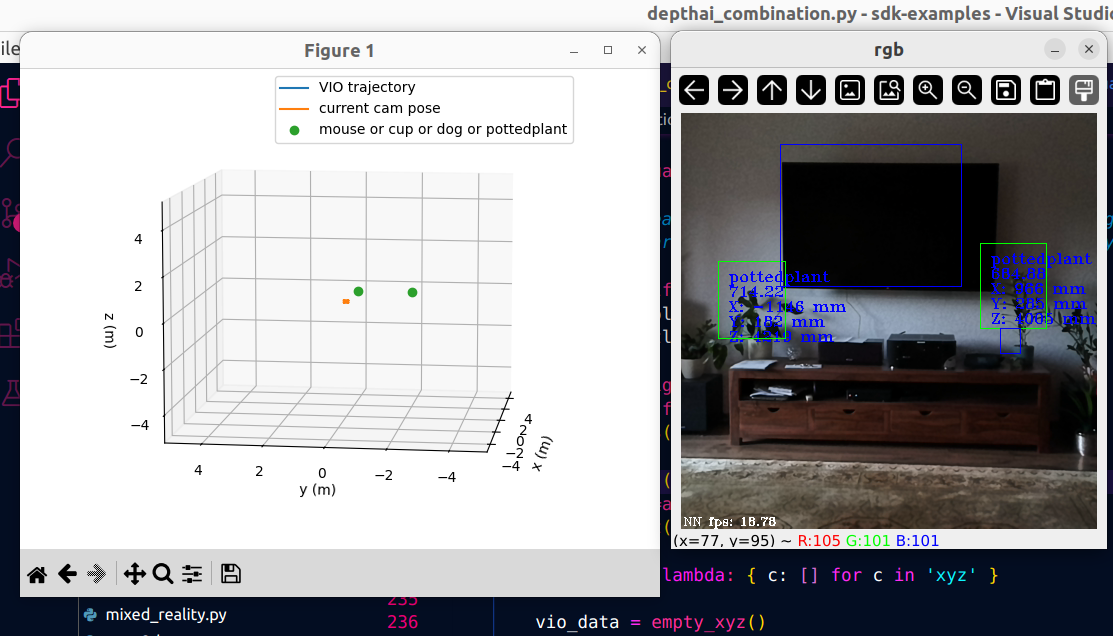
\includegraphics[width=1\linewidth]{images/spectacular_ai_depthai_combination.png}
        \captionof{figure}{Object detection and position estimation with DepthAI}
    \end{minipage}\par
    You can modify the source to detect specific objects. I modified the axes' bounds too so the objects' position is inside the bounding box.
    \item The mixed reality example places a cube in front of the camera's initial position and it stays there (though it shakes a bit sometimes) so you can move the camera around it:\par
    \begin{minipage}{\linewidth}
        \centering
        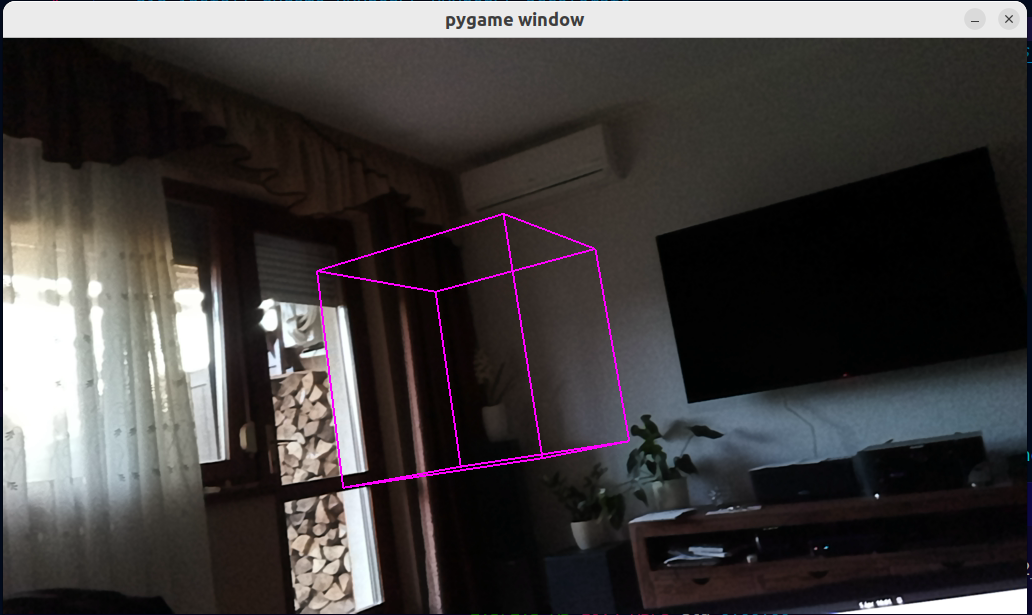
\includegraphics[width=1\linewidth]{images/spectacular_ai_mixed_reality.png}
        \captionof{figure}{Mixed reality cube}
    \end{minipage}\par
    \item According to the documentation, AprilTags can be used too.
    \item Point cloud reconstruction of my room:
    \begin{itemize}
        \item I used the SpectacularAI's \verb|mapping.py| script to create videos with the camera
        \item The \verb|sai-cli process| command creates the keyframes for the NeRF\par
        \begin{minipage}{\linewidth}
            \centering
            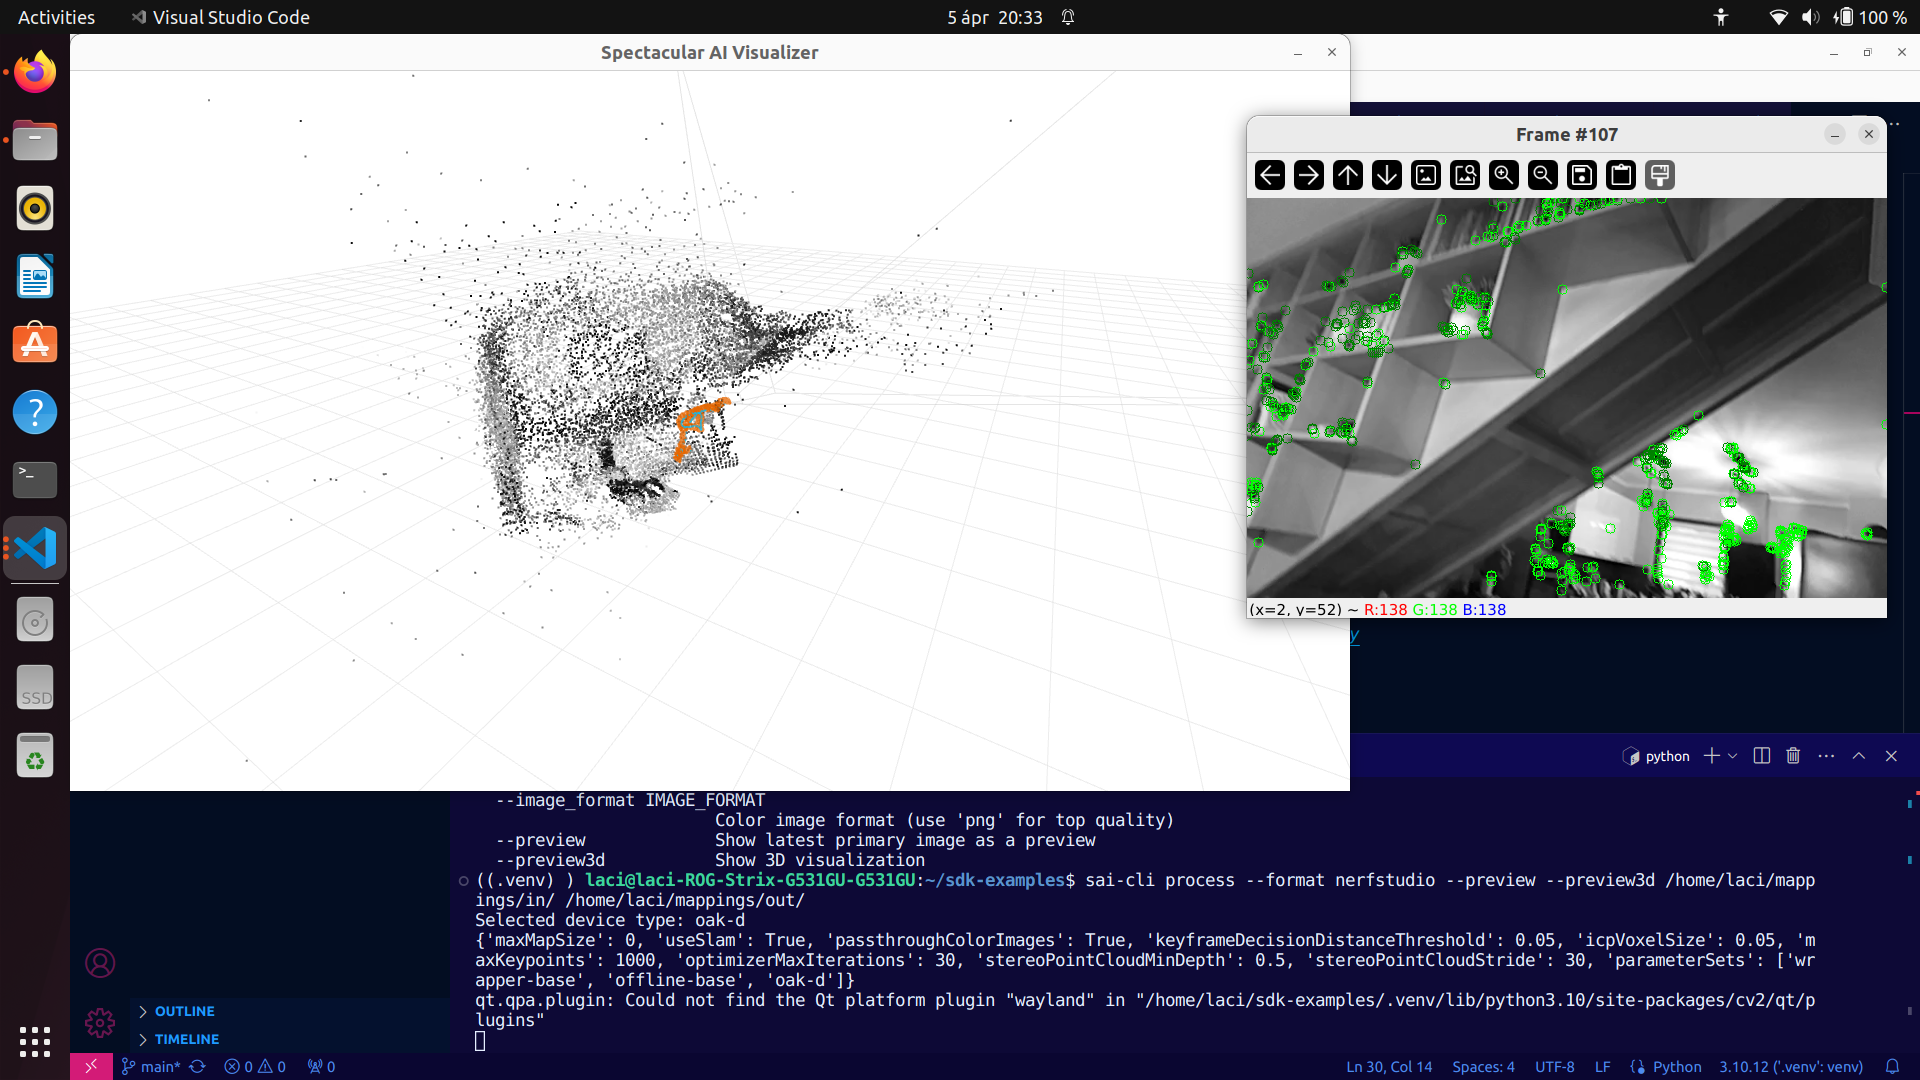
\includegraphics[width=1\linewidth]{images/sai-cli_process.png}
            \captionof{figure}{sai-cli command for creating input for NeRF}
        \end{minipage}\par
        \item Then I used nerfstudio in Docker to create the scene:\par
        \begin{verbatim}
            sudo docker run --gpus all \
            -u $(id -u) \
            -v /home/laci/mappings/:/workspace/ \
            -v /home/laci/.cache/:/home/user/.cache \
            -p 7007:7007 --rm -it \
            --shm-size=1gb dromni/nerfstudio:1.0.3
        \end{verbatim}
        \item You can train the NeRF with the \verb|ns-train ns-train nerfacto --data PATH_TO_DATA| command
        \item You need to have the nVidia driver installed to be able to do this. \par
        \begin{minipage}{\linewidth}
            \centering
            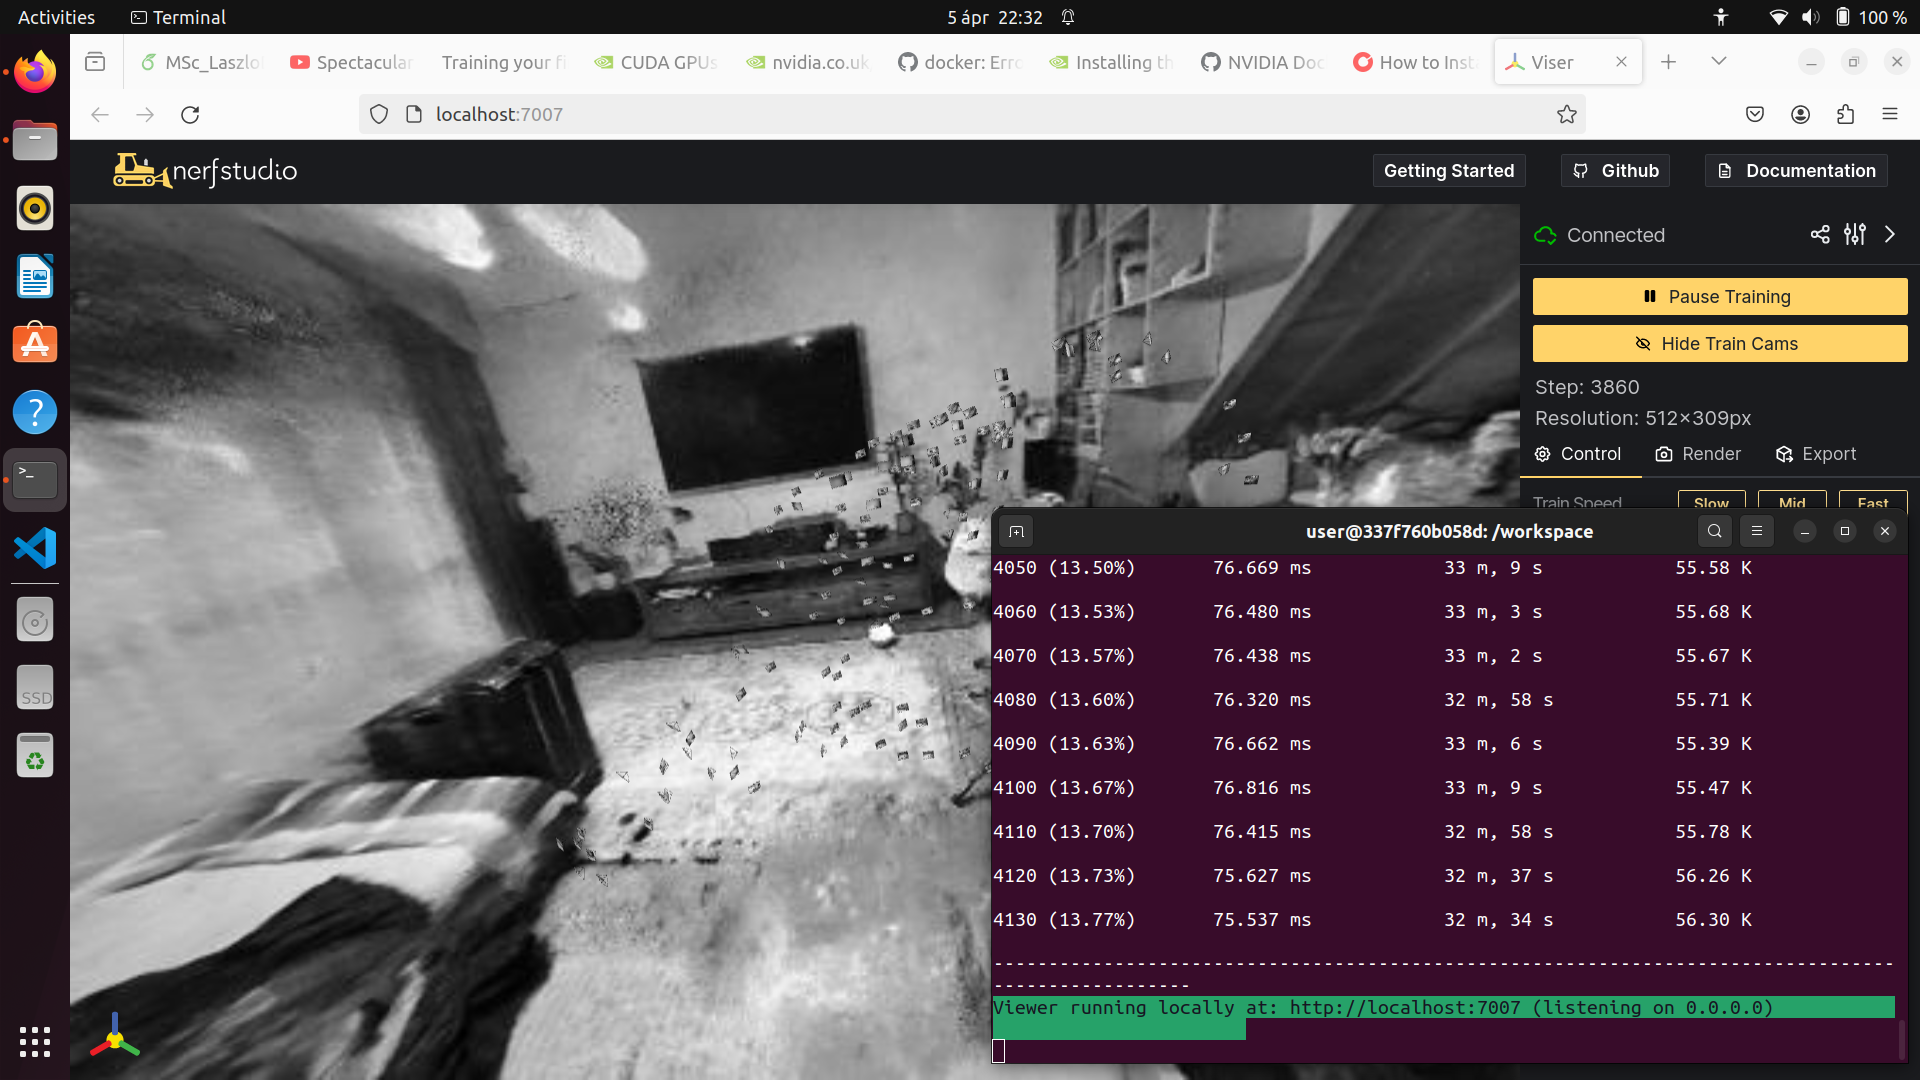
\includegraphics[width=1\linewidth]{images/nerfstudio.png}
            \captionof{figure}{nerfstudio during training}
        \end{minipage}\par
        \item After the training has completed you can view the trained model with:\par
        \begin{verbatim}
            ns-viewer --load-config /workspace/outputs/done/nerfacto/2024-04-05_202416/config.yml
        \end{verbatim}\par
        \begin{minipage}{\linewidth}
            \centering
            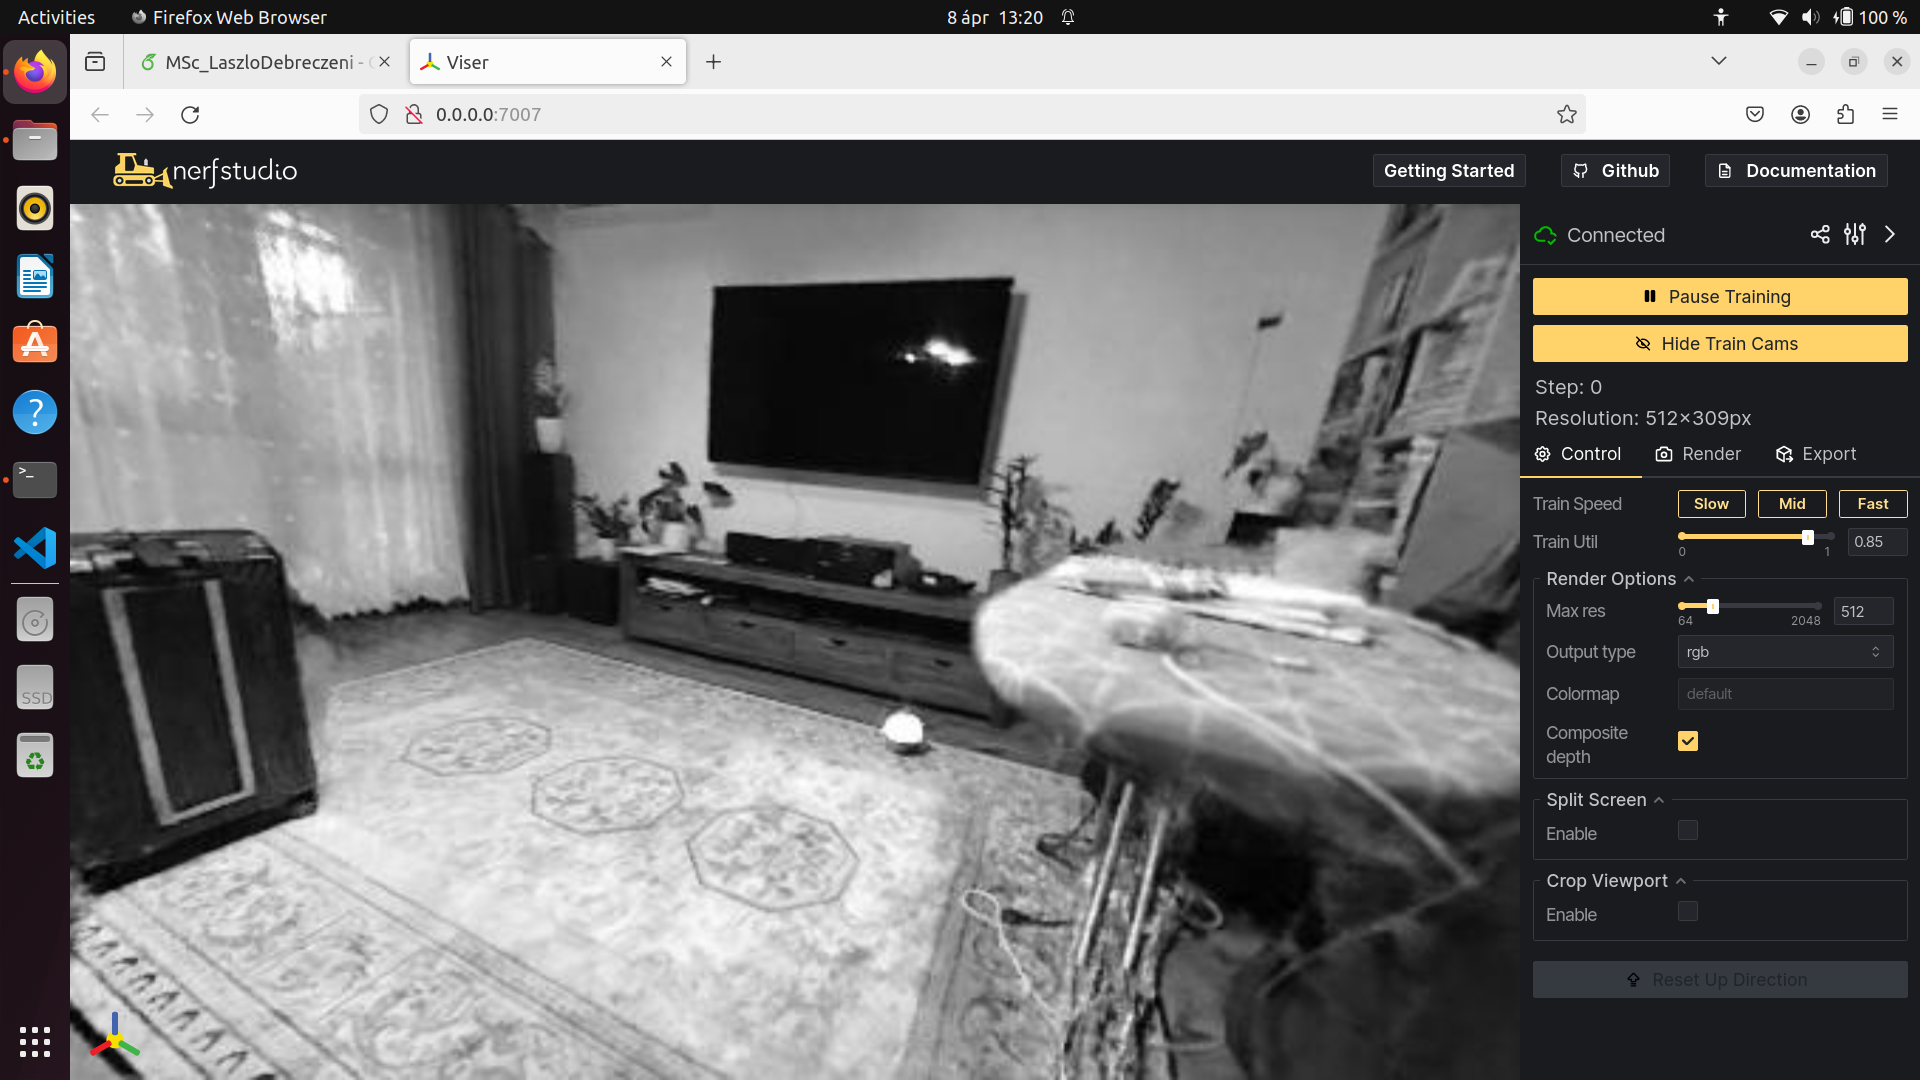
\includegraphics[width=1\linewidth]{images/trained_nerf_karcag1.png}
            \captionof{figure}{Trained NeRF in our living room in Karcag}
        \end{minipage}\par
        \item At some poses the rendering was not so successful because I did not took enough time to shoot the room thoroughly with the camera.
        
    \end{itemize}

    \item It would be interesting to try 3DGS and compare it with nerfstudio: \url{https://github.com/graphdeco-inria/gaussian-splatting}
    
\end{itemize}

\newpage

\section{March 12 -- March 19}

\subsection{What did I do}
\begin{itemize}
    \item DepthAI viewer:\par
    \begin{minipage}{\linewidth}
        \centering
        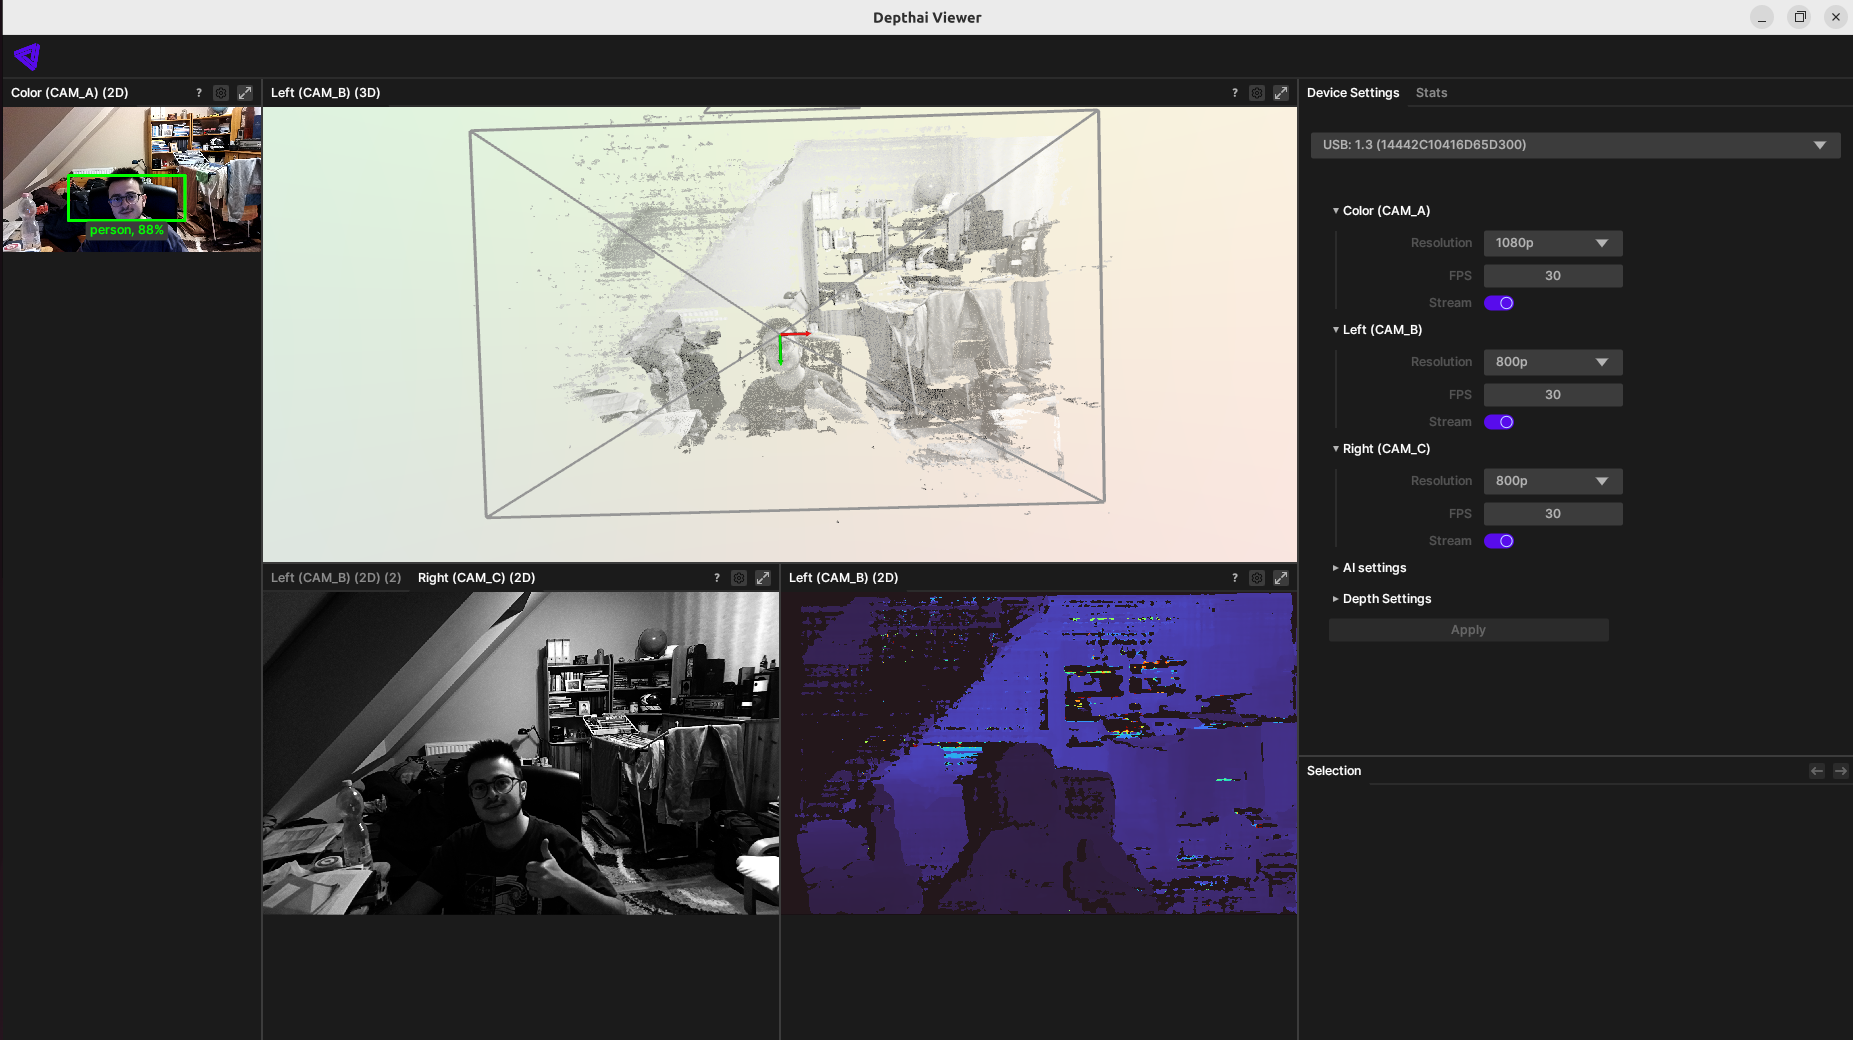
\includegraphics[width=1\linewidth]{depthai_viewer.png}
        \captionof{figure}{DepthAI Viewer}
    \end{minipage}
    \begin{minipage}{\linewidth}
        \centering
        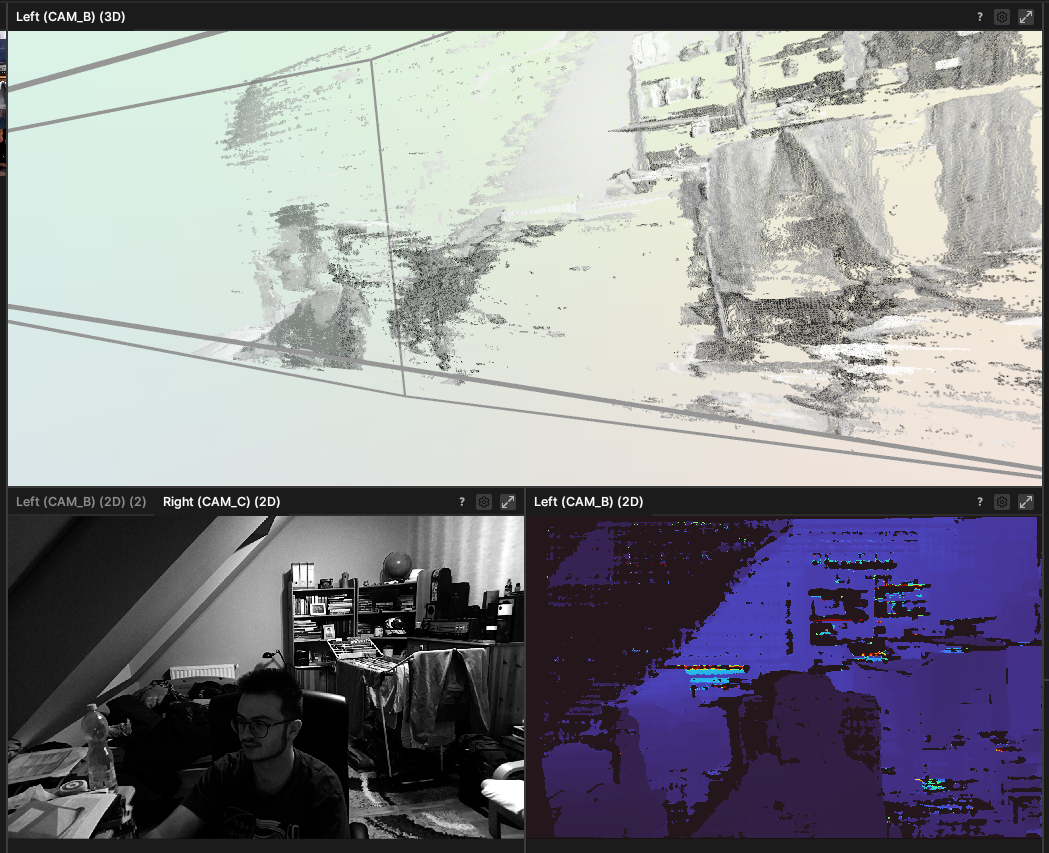
\includegraphics[width=1\linewidth]{depthai_viewer_3d.png}
        \captionof{figure}{DepthAI Viewer 3D reconstruction}
    \end{minipage}
    \item \url{https://docs.luxonis.com/en/latest/pages/slam_oak/}
    \item \url{https://github.com/SpectacularAI/sdk-examples/tree/main/python/oak}
        
\end{itemize}

\subsection{Reading}
Read about 
\begin{itemize}
    \item ORB\_SLAM (\url{https://github.com/raulmur/ORB_SLAM}) \todo[color=green!30]{DONE}
    \item ORB\_SLAM2 (\url{https://github.com/raulmur/ORB_SLAM2})\todo[color=green!30]{DONE}
    \item ORB\_SLAM3 (\url{https://github.com/UZ-SLAMLab/ORB_SLAM3}) \todo[color=green!30]{DONE}
    \item \url{https://webdiis.unizar.es/~raulmur/orbslam/} \todo[color=green!30]{DONE}
\end{itemize}


example citation \cite{Macenski2021}


\subsection{Links}
\begin{itemize}
\item ORB\_SLAM3 with OAKD Pro \url{https://github.com/duncanrhamill/oakd_orbslam3}
\end{itemize}

\subsection{Tasks}
\begin{itemize}
    \item Install the OAK-D camera's dependencies \todo[color=green!30]{DONE}
    \item Try out the DepthAI demos with the OAK-D camera \todo[color=green!30]{DONE}
\end{itemize}

\newpage

\section{March 5 -- March 12}
\begin{itemize}
    \item Turtlebot4 Lite offers maximum current of 1.9 A but Turtlebot4 (the more advanced one) offers only 300 mA \textrightarrow it's kind of weird
    \item Maybe static IP or self-evident hostname for the RPi?
    \item SpectecularAI could be used for large-scale mapping and real-time reconstruction of the area that is mapped with the camera
    \item This could be useful: \url{https://docs.luxonis.com/en/latest/pages/spatial-ai/}
    \item Using custom models on the OAKD: \url{https://docs.luxonis.com/en/latest/pages/model_conversion/}
    \item Running a model on low performance devices (such as the RPi on the Turtlebot4): \url{https://docs.luxonis.com/en/latest/pages/tutorials/local_convert_openvino/}
    \item Camera depth map to point cloud: \url{https://docs.luxonis.com/en/latest/pages/tutorials/device-pointcloud/}
\end{itemize}

\subsection{Reading}
\begin{itemize}
\item read about Turtlebot4 \url{https://turtlebot.github.io/turtlebot4-user-manual/}\todo[color=green!30]{DONE}

\item read about ROSBot2 \url{https://husarion.com/manuals/rosbot/}\todo[color=green!30]{DONE}

\item read about Spectacular AI \url{https://spectacular.ai/}\todo[color=green!30]{DONE}

\item read about DepthAI/OAKD\todo[color=green!30]{DONE}
\begin{itemize}
    \item \url{https://docs.luxonis.com/en/latest/pages/tutorials/first_steps/}
    \item  \url{https://shop.luxonis.com/collections/product-guide}
\end{itemize}

\item read about ROS2 \url{https://github.com/ros2/ros2}\todo[color=blue!30]{IN PROGRESS}


\end{itemize}


\subsection{Tasks}
\begin{itemize}
    \item Install Ubuntu 22\todo[color=green!30]{DONE}
    \item Install ROS2 Humble \url{http://docs.ros.org/en/humble/}\todo[color=green!30]{DONE}
    \item Basic ROS2 tutorials \url{http://docs.ros.org/en/humble/Tutorials.html}\todo[color=blue!30]{IN PROGRESS}
    \item Try out \url{https://turtlebot.github.io/turtlebot4-user-manual/software/turtlebot4_simulator.html}
    \item Try out \url{https://turtlebot.github.io/turtlebot4-user-manual/software/rviz.html}
    \item Try out \url{https://turtlebot.github.io/turtlebot4-user-manual/software/simulation.html}
    \item Try out on the robot: \url{https://turtlebot.github.io/turtlebot4-user-manual/tutorials/}
\end{itemize}

\newpage


\iffalse
\section{EXAMPLE SECTION March 4 -- March 10}
\line(1,0){\linewidth}

\subsection{Current Hurdle/Problem}
\begin{itemize}
\item 
\end{itemize}
\subsection{Reading}
\begin{itemize}
\item 
\end{itemize}

\subsection{Programming}
\begin{itemize}
\item 
\end{itemize}
\subsection{Writing}
\begin{itemize}
\item 
\end{itemize}
\subsection{Insights Gained On the Current Problem}
\begin{itemize}
\item 
\end{itemize}
\subsection{Any Inspiration?}
\begin{itemize}
\item 
\end{itemize}
\subsection{Questions}
\begin{itemize}
\item 
\end{itemize}
\subsection{What's next?}
\begin{itemize}
\item
\end{itemize}
\newpage
\fi

\section{Highlighting Overview}

\colorbox{green}{Successfully completed}\\
\colorbox{yellow}{Pending}\\
\colorbox{orange}{Successfully completed, but didn't solve the problem/but has not effect on the process of the project.}\\
\colorbox{red}{Failed/Not Working}\\
\newpage



\bibliographystyle{plain}
\bibliography{main}

\end{document}
